\begin{homeworkProblem}
  \textbf{( Silueta de la mano)}Para dibujar la silueta de su mano, siga los siguientes pasos:

\begin{enumerate}
    \item[a)] Preparamos una tabla de abcisas y ordenadas usando los siguientes comandos de Matlab:
    \begin{verbatim}
figure('position',get(0,'screensize'))
axes('position',[0 0 1 1])
[x,y] = ginput;
    \end{verbatim}

    \item[b)] Dibuje su mano en un papel y póngalo sobre la pantalla del computador. Use el ratón para seleccionar alrededor de 37 puntos que delineen su mano. Termine la instrucción \texttt{ginput} oprimiendo enter.

    \item[c)] Grafique los puntos $(x, y)$ obtenidos y la mano correspondiente mediante el comando \texttt{plot} de Matlab.

    \item[d)] Implemente el método de splines cúbicos.

    \item[e)] Interpole por separado los puntos $(i, x_i)$ e $(i, y_i)$ mediante splines cúbicos usando su programa.

    \item[f)] Grafique la curva parametrizada que se obtiene.

    \item[g)] Estime el área de su mano usando la fórmula del área de Gauss:
    \[
    A = \frac{1}{2} \left| \sum_{i=1}^{n-1} x_i y_{i+1} + x_n y_1 - \sum_{i=1}^{n-1} x_{i+1} y_i - x_1 y_n \right|
    \]
\end{enumerate}
  \begin{solucion}
    Para construir los splines cúbicos personalizados, primero se parametrizaron las coordenadas en función de un parámetro auxiliar $t$, que en este caso corresponde a la enumeración de los puntos dados. Esto se debe a que la curva no es una función, por ende se describe mediante las coordenadas $(x(t), y(t))$. Luego, se planteó un sistema de ecuaciones tridiagonal para determinar los coeficientes necesarios para la interpolación spline.

El sistema tridiagonal que se resuelve tiene la forma:

\[
\begin{bmatrix}
    a_1 & b_1 & 0 & 0 & \cdots & 0 \\
    b_1 & a_2 & b_2 & 0 & \cdots & 0 \\
    0 & b_2 & a_3 & b_3 & \cdots & 0 \\
    \vdots & \vdots & \vdots & \ddots & \vdots & \vdots \\
    0 & 0 & \cdots & b_{n-3} & a_{n-2} & b_{n-2} \\
    0 & 0 & \cdots & 0 & b_{n-2} & a_{n-1}
\end{bmatrix}
\begin{bmatrix}
    \sigma_1 \\
    \sigma_2 \\
    \sigma_3 \\
    \vdots \\
    \sigma_{n-2} \\
    \sigma_{n-1}
\end{bmatrix}
=
6\begin{bmatrix}
    d_1 \\
    d_2 \\
    d_3 \\
    \vdots \\
    d_{n-2} \\
    d_{n-1}
\end{bmatrix}
\]

donde:

\begin{itemize}
    \item $\sigma_k$ representa los coeficientes de los polinomios de grado tres.
    \item $a_k$ son los elementos de la diagonal principal y se definen como:
    \[
        a_k = 2(h_k + h_{k+1})
    \]
    En este caso, como se parametrizó con la enumeración, se tiene $h_k = 1$, por lo que $a_k = 4$.
    
    \item $b_k$ son los elementos de las diagonales superior e inferior:
    \[
        b_k = h_k
    \]
    Dado que $h_k = 1$, entonces $b_k = 1$.
    
    \item $d_k$ es el término independiente, calculado con diferencias finitas de segundo orden:
    \[
        d_k = \frac{y_{k+1} - y_k}{h_k} - \frac{y_k - y_{k-1}}{h_{k-1}}
    \]
    Como $h_k = 1$, la expresión se simplifica a:
    \[
        d_k = (y_{k+1} - y_k) - (y_k - y_{k-1})
    \]
\end{itemize}

Este sistema se resuelve \textbf{de manera independiente para las coordenadas $x$ y $y$}, permitiendo obtener los valores de $\sigma_k$ que luego se emplean para construir los polinomios cúbicos de interpolación. La solución del sistema se realiza mediante el \textbf{método de Thomas}, una técnica eficiente para resolver sistemas tridiagonales. Con los valores obtenidos, se emplean los polinomios cúbicos de interpolación en cada subintervalo, generando así una curva suave que pasa por los puntos dados.


\begin{lstlisting}
   % Configurar la figura para la entrada de puntos
figure('position', get(0, 'screensize'))
axes('position', [0 0 1 1])
disp('Haga clic en varios puntos y presione Enter cuando termine');

[x, y] = ginput(); % Obtener puntos del usuario
x = [x; x(1)]; % Cerrar el polígono
y = [y; y(1)];

plot(x, y, 'bo-', 'LineWidth', 1.5, 'MarkerSize', 8);
hold on;
disp([x, y]);

% Verificación de puntos mínimos
if length(x) < 4
    error('Se necesitan al menos 4 puntos para la interpolación spline cúbica');
end

% Parametrización
t = 1:length(x);
t_fine = linspace(1, length(x), 100); % Puntos finos para suavidad

% Interpolación con spline de MATLAB
x_spline = spline(t, x, t_fine);
y_spline = spline(t, y, t_fine);
plot(x_spline, y_spline, 'g--', 'LineWidth', 1.5, 'DisplayName', 'Spline de MATLAB');

% Número de incógnitas en el sistema tridiagonal
n = length(x) - 2;

% Calcular segundas diferencias (dx, dy)
dx = 6 * (x(3:end) - 2*x(2:end-1) + x(1:end-2));
dy = 6 * (y(3:end) - 2*y(2:end-1) + y(1:end-2));

% Vectores de la matriz tridiagonal
a = ones(n-1, 1);    % Subdiagonal
b = 4 * ones(n, 1);  % Diagonal principal
c = ones(n-1, 1);    % Superdiagonal

% Resolver el sistema tridiagonal para sigma_x y sigma_y
sigma_x_interior = thomas_solver(a, b, c, dx);
sigma_y_interior = thomas_solver(a, b, c, dy);

% Agregar condiciones de frontera (sigma = 0 en extremos)
sigma_x = [0; sigma_x_interior; 0];
sigma_y = [0; sigma_y_interior; 0];

% Interpolación personalizada usando splines cúbicos
x_int = [];
y_int = [];
for i = 1:length(x)-1
    t_i = linspace(t(i), t(i+1), 10);
    for k = 1:length(t_i)
        x_val = spline_polinomios(t_i(k), t(i), t(i+1), x(i), x(i+1), sigma_x(i), sigma_x(i+1));
        y_val = spline_polinomios(t_i(k), t(i), t(i+1), y(i), y(i+1), sigma_y(i), sigma_y(i+1));
        x_int = [x_int, x_val];
        y_int = [y_int, y_val];
    end
end

% Graficar resultado personalizado
plot(x_int, y_int, 'r-', 'LineWidth', 1.5, 'DisplayName', 'Spline Personalizado');

% Cálculo del área con la fórmula de Gauss
n_points = length(x);
sum1 = 0;
sum2 = 0;
for i = 1:n_points-1
    sum1 = sum1 + x(i) * y(i+1);
    sum2 = sum2 + x(i+1) * y(i);
end
sum1 = sum1 + x(n_points) * y(1); % Cerrar polígono
sum2 = sum2 + x(1) * y(n_points);

Ar = 0.5 * abs(sum1 - sum2);
disp(['Área calculada: ', num2str(Ar)]);

% Configurar la gráfica
title('Interpolación Spline Cúbica');
xlabel('X'); ylabel('Y');
grid on;
legend('Puntos Originales', 'Spline de MATLAB', 'Spline Personalizado', 'Location', 'best');
hold off;

area_correcta = polyarea(x, y);
disp(['Área con polyarea: ', num2str(area_correcta)]);

% --- Función para resolver sistemas tridiagonales con el algoritmo de Thomas ---
function x = thomas_solver(a, b, c, d)
    n = length(d);
    cp = c;   
    dp = d;   
    bp = b;   
    
    % Eliminación hacia adelante
    for i = 2:n
        m = a(i-1) / bp(i-1);
        bp(i) = bp(i) - m * cp(i-1);
        dp(i) = dp(i) - m * dp(i-1);
    end
    
    % Sustitución hacia atrás
    x = zeros(n, 1);
    x(n) = dp(n) / bp(n);
    for i = n-1:-1:1
        x(i) = (dp(i) - cp(i) * x(i+1)) / bp(i);
    end
end

% --- Función de interpolación spline cúbica ---
function q = spline_polinomios(t, t_k, t_k1, y_k, y_k1, sigma_1, sigma_2)
    term1 = (sigma_1 / 6) * ((t_k1 - t)^3 - (t_k1 - t));
    term2 = (sigma_2 / 6) * ((t - t_k)^3 - (t - t_k));
    term3 = y_k * (t_k1 - t);
    term4 = y_k1 * (t - t_k);
    q = term1 + term2 + term3 + term4;
end

\end{lstlisting}
La implementación del código da un área de $0.10296 u^2$ para la mano de Sandra y un área de $0.09439 u^2$ para la de Andrés. A continuación, se comparan los resultados gráficos:

\begin{figure}[H]
    \centering
    \begin{minipage}{0.48\textwidth}
        \centering
        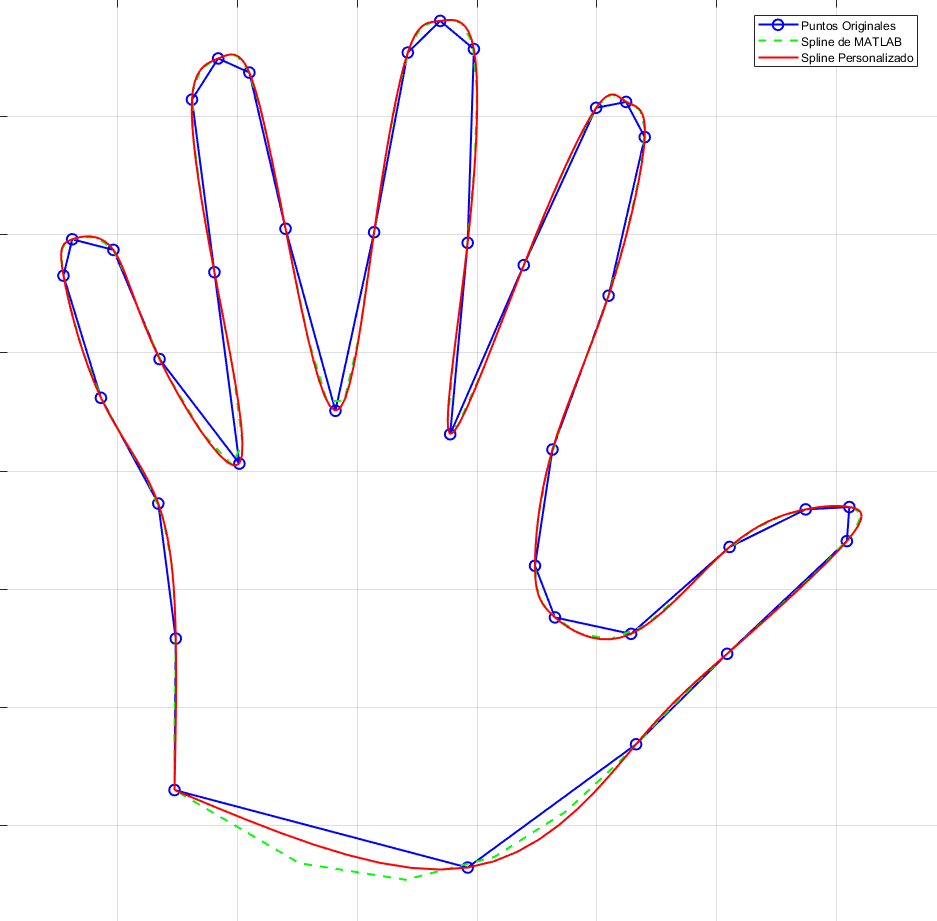
\includegraphics[width=\textwidth]{Figures/mano final.png} % Cambia por el nombre correcto
        \caption{Spline de la mano de Sandra.}
        \label{fig:spline_sandra}
    \end{minipage}
    \hfill
    \begin{minipage}{0.48\textwidth}
        \centering
        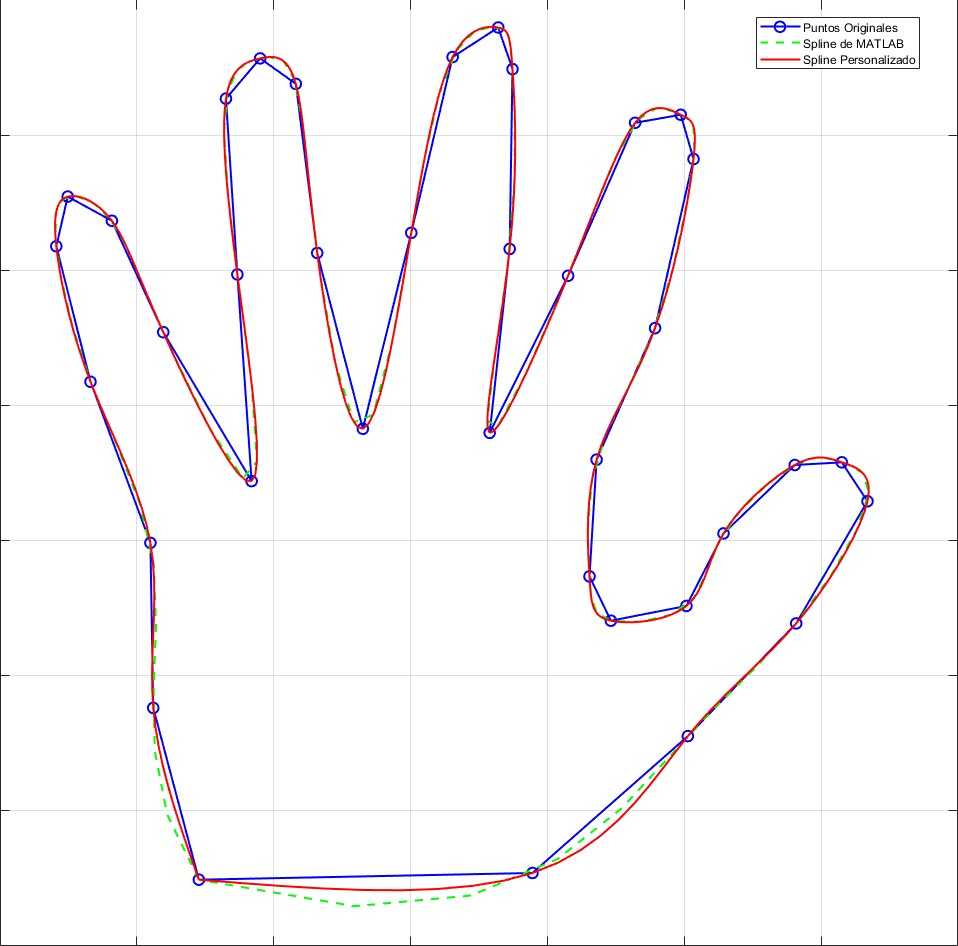
\includegraphics[width=\textwidth]{Figures/mano Andres.jpg} % Cambia por el nombre correcto
        \caption{Spline de la mano de Andrés.}
        \label{fig:spline_andres}
    \end{minipage}
\end{figure}

Los gráficos muestran la interpolación realizada mediante splines cúbicos. En cada imagen, los trazos azules representan los puntos originales, la curva roja corresponde al spline cúbico implementado manualmente y la curva verde representa la interpolación generada por MATLAB.

La interpolación realizada con splines cúbicos genera una aproximación suave y continua a partir de los puntos dados, evitando las oscilaciones bruscas que podrían aparecer con otros métodos, como la interpolación polinómica global. La implementación personalizada resuelve un sistema tridiagonal para obtener las segundas derivadas en los puntos de control, garantizando una transición fluida entre segmentos. Esto se traduce en una curva interpolada que respeta la forma general de los datos originales sin generar artefactos inesperados.  

Al comparar la interpolación con el spline de MATLAB, se pueden notar ligeras diferencias en ciertos tramos. Esto puede deberse a la forma en que cada método maneja las condiciones de frontera y distribuye los puntos interpolados. MATLAB emplea una parametrización interna que puede afectar la forma final de la curva, mientras que la interpolación personalizada usa una parametrización directa basada en la posición secuencial de los puntos. Como resultado, aunque ambas curvas siguen la misma estructura general, hay pequeñas variaciones en la forma en que se suavizan ciertas transiciones. Estas diferencias pueden observarse con mayor claridad en la siguiente figura:  

\begin{figure}[H] % Asegura que la imagen aparezca en la posición deseada
    \centering
    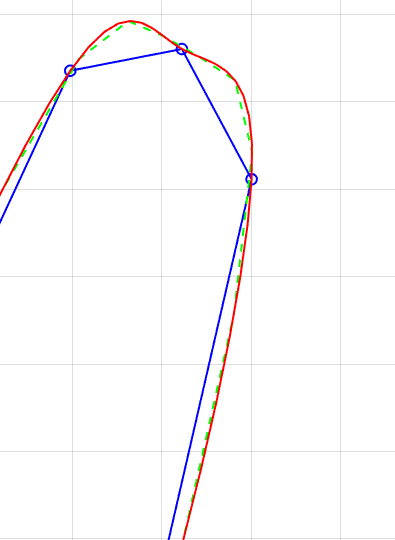
\includegraphics[width=0.5\textwidth]{Figures/pulgar.png} % Cambia el nombre del archivo
    \caption{Vista ampliada de la gráfica en un dedo.}
    \label{fig:detalle_dedo}
\end{figure}  

En términos de exactitud, ambas interpolaciones ofrecen una aproximación adecuada a la forma original. La interpolación manual proporciona una representación fiel y coherente con los datos ingresados, manteniendo una curva suave que se ajusta a la estructura esperada. Aunque hay pequeñas diferencias con MATLAB, estas no implican una pérdida de precisión significativa, sino más bien una variación en la forma en que cada método interpola los segmentos individuales.  

Para visualizar mejor cada interpolación, se presentan las tres gráficas por separado. En estas representaciones individuales, se puede apreciar con mayor claridad cómo se ajusta cada spline a los puntos originales.
\begin{figure}[H]
    \centering
    \begin{minipage}{0.48\textwidth}
        \centering
        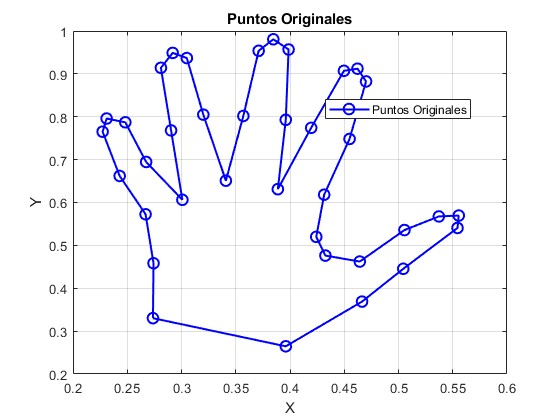
\includegraphics[width=\textwidth]{Figures/puntos originales.jpg} % Cambia por el nombre correcto
        \label{fig:imagen1}
    \end{minipage}
    \hfill
    \begin{minipage}{0.48\textwidth}
        \centering
        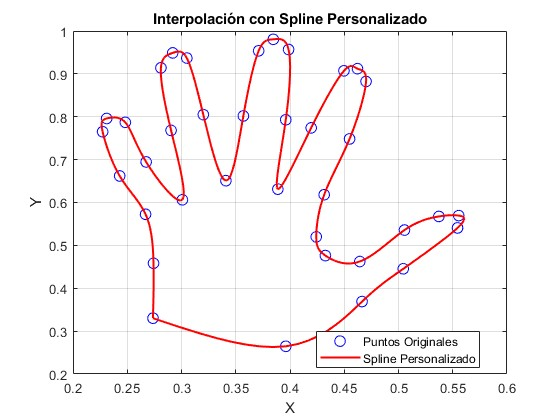
\includegraphics[width=\textwidth]{Figures/interpolacion propia.png} % Cambia por el nombre correcto
        \label{fig:imagen2}
    \end{minipage}

    % Imagen inferior
    \vfill
    \begin{minipage}{0.6\textwidth}
        \centering
        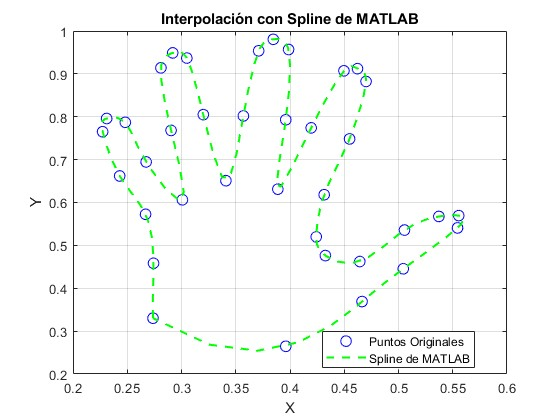
\includegraphics[width=\textwidth]{Figures/interpolacion de matlab.jpg} % Cambia por el nombre correcto
        \label{fig:imagen3}
    \end{minipage}
\end{figure}

  \end{solucion}
\end{homeworkProblem}
